\documentclass[
	format=sigconf,
	review=false]{acmart}

\usepackage{booktabs} % For formal tables
\usepackage{fancyref}
\usepackage{subcaption}

% ----------------------------------
% Submission site:
% https://cmt3.research.microsoft.com/DSMM2017/
%

% Copyright
%\setcopyright{none}
%\setcopyright{acmcopyright}
%\setcopyright{acmlicensed}
\setcopyright{rightsretained}
%\setcopyright{usgov}
%\setcopyright{usgovmixed}
%\setcopyright{cagov}
%\setcopyright{cagovmixed}


% DOI
\acmDOI{10.475/123_4}

% ISBN
\acmISBN{123-4567-24-567/08/06}

%Conference
\acmConference[DSMM'17]{ACM Data Science for Macro-Modeling with Financial and Economic Datasets}{May 2017}{Chicago, USA} 
\acmYear{2017}
\copyrightyear{2017}

\title{Ranking Sentences Describing Relationships Between Financial Entities by Relevance}

%\author{
%	\begin{tabular*}{0.7\textwidth}{cc}
%		\LARGE\sffamily Lorenz Tim & \LARGE\sffamily Nome2 \\
%		\large\normalfont Department1 & \large\normalfont Department2 \\
%		School1 & School2
%	\end{tabular*}
%}

%\LARGE\sffamily Author
%\large\normalfont Affiliation

\author{
	Tim Repke, Michael Loster, Ralf Krestel, Felix Naumann
}
\affiliation{%
	\institution{Hasso-Plattner-Institute}
	\city{Potsdam}
	\country{Germany}
}
\email{firstname.lastname@hpi.de}
%\affiliation{aksdj}
% The default list of authors is too long for headers}
\renewcommand{\shortauthors}{T. Repke et al.}


\begin{document}

%\begin{abstract}
%This paper provides a sample of a \LaTeX\ document which conforms,
%somewhat loosely, to the formatting guidelines for
%.ACM SIG Proceedings.\footnote{This is an abstract footnote}
%\end{abstract}

%
% The code below should be generated by the tool at
% http://dl.acm.org/ccs.cfm
% Please copy and paste the code instead of the example below. 
%
\begin{CCSXML}
<ccs2012>
 <concept>
  <concept_id>10010520.10010553.10010562</concept_id>
  <concept_desc>Computer systems organization~Embedded systems</concept_desc>
  <concept_significance>500</concept_significance>
 </concept>
 <concept>
  <concept_id>10010520.10010575.10010755</concept_id>
  <concept_desc>Computer systems organization~Redundancy</concept_desc>
  <concept_significance>300</concept_significance>
 </concept>
 <concept>
  <concept_id>10010520.10010553.10010554</concept_id>
  <concept_desc>Computer systems organization~Robotics</concept_desc>
  <concept_significance>100</concept_significance>
 </concept>
 <concept>
  <concept_id>10003033.10003083.10003095</concept_id>
  <concept_desc>Networks~Network reliability</concept_desc>
  <concept_significance>100</concept_significance>
 </concept>
</ccs2012>  
\end{CCSXML}

\ccsdesc[500]{Computer systems organization~Embedded systems}
\ccsdesc[300]{Computer systems organization~Redundancy}
\ccsdesc{Computer systems organization~Robotics}
\ccsdesc[100]{Networks~Network reliability}

% We no longer use \terms command
%\terms{Theory}

%\keywords{ACM proceedings, \LaTeX, text tagging}

\settopmatter{printccs=false, printacmref=false, printfolios=false}

\maketitle

\section{Introduction}
Efficiently identifying relations between companies based on 10k filings ... support analysts.

FEIII Challenge 2017\footnote{\url{https://ir.nist.gov/feiii/}}

% from webpage: Given a 10-K filing, an analyst asks, does Company Y, mentioned in this filing, play the role R with respect to filing Company X? Rather than simply answering "yes" or "no", a system responds by providing all the mentions of Company Y in Company X's 10-K filing, with context sentences. These triples are then in ordered by the likelihood that the context accurately defines the relationship or role R between X and Y.

\section{Description of the Data}


source of sentences (10K/Q filings, 25 documents)

\subsection{Inter Annotator Agreement}
The quality of annotations is estimated using Cohen's kappa. The inter annotator agreement (IAA) between two experts is defined as
$$
\kappa = \frac{p_0-p_e}{1-p_e},
$$
where $p_0$ is the proportion of labels with agreement, and $p_e$ the statistical chance of random agreement.

\begin{figure}
	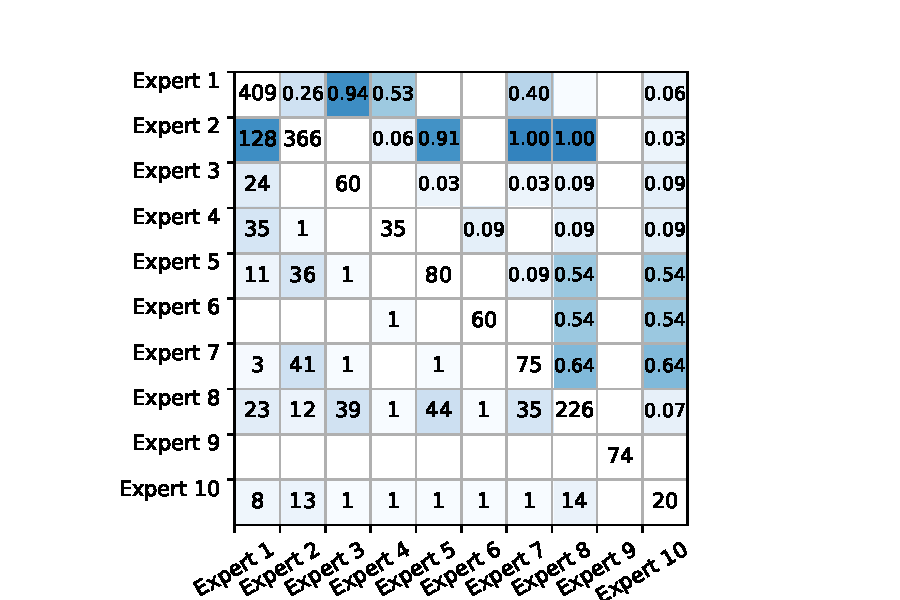
\includegraphics[width=\linewidth]{iaa}
	\caption{$\kappa$ IAA (upper triangular matrix), number of commonly rated triples (lower triangular matrix), and number of ratings (diagonal matrix)}
	\label{fig:iaa}
\end{figure}

\Fref{fig:iaa} shows the $\kappa$ for each pair of experts, as well as the number of overlapping labels. Most triplets (60\%) aren't represented in this figure, since they only received a rating by one expert and very few by more than two. The weighted average of $\overline{k}<0.5$ and few overlapping annotations are not ideal for a reliable development and evaluation of a system. For all experiments each triplet's rounded average rating is considered.

\subsection{Preparing the Dataset}

avg and clip annotator scores, lemmatise sentences, tfidf bow

\section{Ranking Algorithm}

\section{Evaluation and Conclusion}
The system's performance is measured by the Normalised Discounted Cumulative Gain (NDCG). The rank at position $p$ is calculated by
\begin{equation}
NDCG_p = \frac{DCG_p}{IDCG_p},\;
DCG_p = rel_1 + \sum_{i=2}^{p} \frac{rel_i}{\log_2(i+1)}
\end{equation}
where $DCG_p$ is the Discounted Cumulative Gain (DCG) when ordering items based on a given score, $IDCG_p$ the ideal DCG, and $rel_i$ the relevance of an item at position $i$ as depicted by the experts.



\bibliographystyle{ACM-Reference-Format}
\bibliography{sigproc} 

\end{document}
